\documentclass[12pt,letterpaper]{article}
\usepackage[utf8]{inputenc}
\usepackage{amsmath}
\usepackage{amsfonts}
\usepackage{amssymb}
\usepackage{graphicx}
\usepackage[left=2cm,right=2cm,top=2cm,bottom=2cm]{geometry}
\author{Kris Garrett}
\title{Tycho 2 User Guide (Draft)}
\begin{document}
\maketitle


\section{Introduction}
Tycho 2 is a reworking of a code named Tycho written by Shawn Pautz around the year 2000.
The original code solved a linear, kinetic, transport equation on an unstructured, 3D tetrahedral mesh and was parallelized via MPI.
The original code was made to test the performance of transport sweeps which will be subsequently described.

Tycho 2 solves the same equation with some additions.
The new code adds energy dependence to the calculations to give realistic computational results for cases with several energy groups.
The code is implemented in MPI and OpenMP and uses only open source software and libraries to generate meshes and compile.







\section{Compiling and running the code}
The code is split into the main executable named {\tt sweep.x} and several utilities dealing with meshes in the {\tt util} directory.
All the code requires a C++11 compliant compiler.
The main program, sweep.x, also requires MPI and OpenMP to compile.
The utilities in the {\tt util} directory are all serial and hence do not require MPI or OpenMP.
However, depending on the utility, various libraries are needed.
These will be described below.


\subsection{Compiling sweep.x}
\paragraph{Quick step guide}
\begin{itemize}
\item Copy {\tt make.inc.example} to {\tt make.inc}
\item Set {\tt ASSERT} and {\tt MPICC} in the file {\tt make.inc}
\item Type {\tt make} to build {\tt sweep.x}
\end{itemize}

\paragraph{Details}
To compile {\tt sweep.x}, first copy {\tt make.inc.example} to {\tt make.inc} in the main project directory.
The file {\tt make.inc} contains the two user definable parts for the build process.
The first user definable parameter is {\tt ASSERT}.
If {\tt ASSERT = 1}, then the code will run much slower since bounds checking is performed on all the multidimensional arrays.

The second user definable parameter is your compiler information, which is set in {\tt MPICC}.
In this, you name the MPI compiler wrapper and any features of the compilation you want such as optimization and debugging symbols.
You must enable C++11 and OpenMP for your compiler.
For an optimized compile using GCC, I usually set {\tt mpicxx -O3 -Wall -Wextra -pedantic -std=c++11 -fopenmp}.
This compile command is optimized to level 3, spits out as many warnings as possible, enables C++11 features, and enables OpenMP.

The last step is to type {\tt make} to build the main executable.
The {\tt Makefile} will include the variables set in {\tt make.inc}.
All the object files will be stored in the {\tt build} directory and the executable, {\tt sweep.x}, will be created in the main project directory.


\subsection{Compiling the utilities}
The util directory contains several utilities for creating and partitioning meshes that sweep.x will use.
When you clone Tycho 2 from github, you should get several files in the util directory.
\begin{itemize}
\item {\tt cube\_no\_mesh.hdf} -- File containing a cube's geometry.  The cube is a 100x100x100 cube.  This can be opened by certain CAD programs to be meshed.
\item {\tt cube-<N>.cgns} -- CGNS file formatted tetrahedral meshes of {\tt cube\_no\_mesh.hdf} where $N$ is the number of cells in the mesh.
\item {\tt cube-<N>.smesh} -- The same meshes as given by {\tt cube-<N>.cgns}, just in a file format made for Tycho 2 that does not require any library dependencies to be read.
\item {\tt CreateGaussLegendre.py} -- This is a Python script used to create the Gauss Legendre quadrature in the main code.
\item {\tt MakeTet.py} -- This is a Python script used to make one tetrahedron in the smesh file format.
\item {\tt CreateRegularMesh.cc} -- Creates a regular Cartesian mesh and then each hexahedron is split into Tetrahedra.
\item {\tt MoabToSerialMesh.cc} -- Uses the MOAB mesh library to read in a common mesh format (such as CGNS, HDF5, NetCDF, etc) and convert it to the smesh file format.
\item {\tt ParallelMeshToMoab.cc} -- Converts the pmesh file format into a file format that the Visit visualization tool can read.
\item {\tt PartitionColumns.cc} -- Partitions an smesh into a pmesh by columns.
\item {\tt RefineSerialMesh.cc} -- Refines each tetrahedron in an smesh into 8 tetrahedra.
\item {\tt SerialMeshToMoab.cc} -- Converts the smesh file format into a file format that the Visit visualization tool can read.
\item {\tt SerialToParallelMesh.cc} -- Partitions an smesh using the Metis partitioning library.
\end{itemize}

\paragraph{Creating a pmesh}
To run the main executable {\tt sweep.x}, you must supply a pmesh as an argument to the executable.
Several smesh files containing meshes of cubes are supplied, but it is also possible to supply your own mesh.
Either the PartitionColumns or SerialToParallelMesh utility must be used to convert an smesh file into a pmesh file.
PartitionColumns requires no library dependencies and SerialToParallelMesh requires the Metis partitioning library.

\paragraph{Creating your own mesh}
If you wish to supply your own mesh, you will need to convert your mesh into an smesh.
This can be done using the MoabToSerialMesh utility which requires the MOAB mesh library.
MOAB can read several mesh file format, but extra libraries may have to be included in the build process for your mesh format.

\paragraph{Visualization}
If you wish to visualize either an smesh or pmesh, you will use either the SerialMeshToMoab or ParallelMeshToMoab utilities.
These require the MOAB mesh library, but no other dependencies are required.
SerialMeshToMoab will create a .vtk file that can be read by Visit.
ParallelMeshToMoab will create a .vtk file for each partition of the pmesh and a .visit file linking all the .vtk files together.
You can then read the .visit file in Visit to visualize the mesh and its partitions.

\paragraph{The build process}
The build process is almost the same as for the main executable.
\begin{itemize}
\item Copy {\tt make.inc.example} to {\tt make.inc}
\item Set {\tt CPP} in the file {\tt make.inc}
\item Set any of the library directories needed by the utilities you will build
\item Type {\tt make <name of utility>}.  For instance {\tt make PartitionColumns} will create the executable {\tt PartitionColumns.x}.  Typing {\tt make} without a target will attempt to build all the utilities.
\end{itemize}


\subsection{Running sweep.x}
To run {\tt sweep.x}, type {\tt ./sweep.x <.pmesh file> <input.deck file>}.
This requires that you have created a pmesh as described in the previous section and you have copied {\tt input.deck.example} to {\tt input.deck} (or any other name you prefer).
In {\tt input.deck}, you have the following options to set.
\begin{itemize}
\item {\tt snOrder} -- Order of the angular quadrature.  This can be any even number from 2 to 30.
\item {\tt iterMax} -- Maximum number of iterations for source iteration
\item {\tt errMax} -- Tolerance for the relative error for source iteration
\item {\tt maxCellsPerStep} -- Maximum number of of cell/angle pairs to compute for $\Psi$ before communication via MPI
\item {\tt intraAngleP} -- This can be 0, 1, 2, 3, or 4 for random, b-level, BFDS, DFDS, and DFHDS
\item {\tt interAngleP} -- This can be 0, 1, or 2 for interleaved, globally prioritized, and locally prioritized
\item {\tt nGroups} -- Number of energy group.  Should be 1 or greater.
\item {\tt SweepType} Type of sweeper to use.  Possible values are commented in the input.deck file.
\end{itemize}
An example {\tt run.sh} script is supplied which will create a pmesh with 1 partition and run {\tt sweep.x} in serial.










\section{The underlying mathematics}
\subsection{The equation}
Tycho 2 solves the following kinetic equation with isotropic scattering
\begin{equation} \label{eq:main}
\Omega \cdot \nabla_x \Psi(x,\Omega,E) + \sigma_t \Psi(x,\Omega,E) = \frac{\sigma_s}{4\pi} \int_{\mathbb{S}^2} \Psi(x,\Omega',E) d\Omega' + Q(x,\Omega,E).
\end{equation}
The function $\Psi$ is the unknown, $\sigma_t$ and $\sigma_s$ are the total and scattering cross sections with $\sigma_t > \sigma_s$ and are constant.
The function $Q$ is a known source.

The independent variables are:
\begin{itemize}
\item Space -- $x \in \mathcal{D} \subset \mathbb{R}^3$,
\item Direction -- $\Omega \in \mathbb{S}^2$ (the unit sphere), 
\item Energy -- $E \in \mathbb{R}^{\geq 0}$.
\end{itemize}
Notice the equation is dependent on energy, but the different energies are not coupled.
This is done on purpose since the goal is to test sweeping strategies which are uncoupled in energy.

For the purpose of simpler notation, define
\begin{equation}
\Phi(x,E) = \int_{\mathbb{S}^2} \Psi(x,\Omega',E) d\Omega'
\end{equation}
to get the equivalent equation
\begin{equation} \label{eq:main1}
\Omega \cdot \nabla_x \Psi(x,\Omega,E) + \sigma_t \Psi(x,\Omega,E) = \frac{\sigma_s}{4\pi} \Phi(x,E) + Q(x,\Omega,E).
\end{equation}


\subsection{Method of discretization}
Equation \eqref{eq:main1} is discretized using: discontinuous Galerkin (DG) with linear elements in $x$, discrete ordinates in $\Omega$, and energy groups in $E$.


\paragraph{Energy discretization.}
Since equation~\eqref{eq:main1} is not coupled in energy, the method of discretization of $E$ does not matter.
However, it is typical to discretize $E$ into energy groups.
Hence, the discretization in energy is denoted by $E_g$ where $g$ is an integer indexing the energy group (though any other discretization is fine).
\begin{equation}
\Omega \cdot \nabla_x \Psi_g(x,\Omega) + \sigma_t \Psi_g(x,\Omega) = \frac{\sigma_s}{4\pi} \int_{\mathbb{S}^2} \Psi_g(x,\Omega') d\Omega' + Q_g(x,\Omega).
\end{equation}


\paragraph{Angle discretization.}
Angle is discretized via discrete ordinates, which is often denoted as S$_N$ where $N$ is the order of the discretization.
Tycho 2 implements the Chebyshev-Legendre quadrature of the sphere.
This involves a Cartesian product of $N$ Legendre nodes on the z-axis and $2N$ equally spaced points on the circle for each Legendre node.
The weights are proportional to the weights of the Legendre quadrature and scaled to sum to $4\pi$.
The nodes and weights will be denoted by $\Omega_q$ and $w_q$, where $q$ stands for the quadrature index.

Equation~\eqref{eq:main} becomes
\begin{equation}
\Omega_q \cdot \nabla_x \Psi_{qg}(x) + \sigma_t \Psi_{qg}(x) = 
\frac{\sigma_s}{4\pi} \sum_{q'=0}^{2N^2-1} w_{q'} \Psi_{q'g}(x) + Q_{qg}(x).
\end{equation}
Equation~\eqref{eq:main1} becomes
\begin{equation}
\Omega_q \cdot \nabla_x \Psi_{qg}(x) + \sigma_t \Psi_{qg}(x) = 
\frac{\sigma_s}{4\pi} \Phi_{g}(x) + Q_{qg}(x),
\end{equation}
where
\begin{equation}
\Phi_g(x) = \sum_{q'=0}^{2N^2-1} w_{q'} \Psi_{q'g}(x).
\end{equation}
Below is a depiction of the quadrature nodes on the sphere.

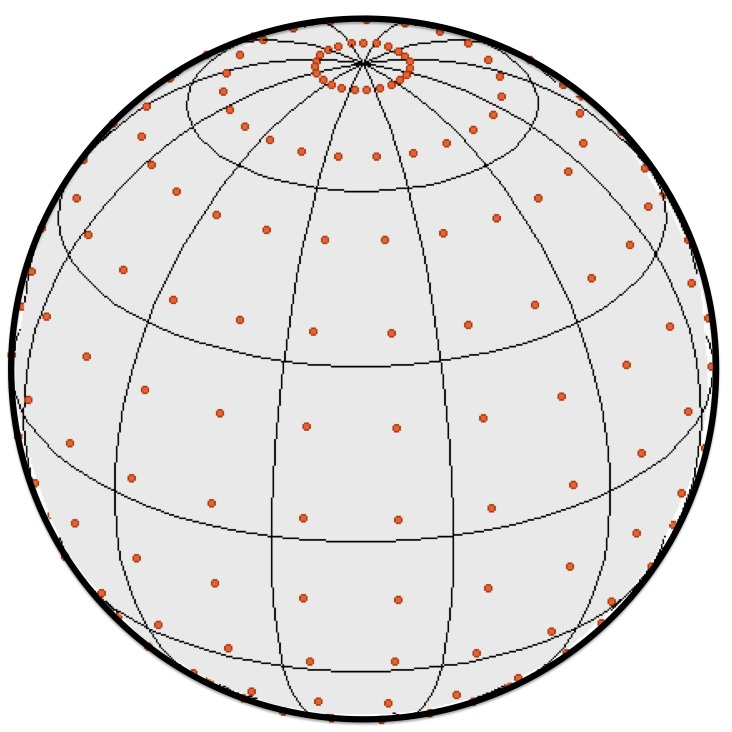
\includegraphics[scale=0.5]{chebyshev-legendre.jpg}


\paragraph{Spatial discretization.}
Since source iteration is used to converge the RHS of equation~\eqref{eq:main}, it will be easier to show the equations for the simpler problem
\begin{equation}
\Omega_q \cdot \nabla_x \Psi_{qg}(x) + \sigma_t \Psi_{qg}(x) = Q_{qg}(x).
\end{equation}
In this formulation, the scattering term has been absorbed into the source $Q_{qg}(x)$.

Space is discretized via linear DG.
In each tetrahedral cell $C_i$, define basis functions $b_{ik}|_{k=0}^3$ to be linear interpolation functions with 
\begin{equation}
b_{ik} = \begin{cases}
1, \textrm{ at vertex } k \textrm{ of cell } C_i \\
0, \textrm{ at other vertices of cell } C_i
\end{cases}.
\end{equation}
Also, define 
\begin{equation}
\Psi^h|_{C_i} = \sum_k \Psi_{ik} b_k.
\end{equation}

Then the DG formulation is derived by starting with the equation
\begin{equation} \label{eq:sweep}
\Omega \cdot \nabla_x \Psi(x) + \sigma_t \Psi(x) = Q(x),
\end{equation}
where the subscripts $q,g$ are implicit.
Then multiply by test function $b_j$ in cell $C_i$ and integrate to get
\begin{equation}
\int_{C_i} \Omega \cdot \nabla_x \Psi b_j dx + \int_{C_i} \sigma_t \Psi b_j dx = \int_{C_i} Q b_j dx.
\end{equation}
Then use integration by parts on the first integral to get
\begin{equation}
-\int_{C_i} \Omega \cdot \nabla_x b_j \Psi dx + 
\sum_k \int_{F_{ik}} (\Omega \cdot \nu_k) b_j \hat{\Psi}^{(k)} dA + 
\int_{C_i} \sigma_t \Psi b_j dx = \int_{C_i} Q b_j dx.
\end{equation}
Here, $k$ indexes over the faces $F_{ik}$ of cell $i$, and $\nu_k$ is the outward normal to face $F_{ik}$.
The only thing left to define is the numerical flux $\hat{\Psi}^{(k)}$.
Since $\Psi$ is discontinuous at the faces, this is not well defined and must be defined by the numerical method.
We use the upwind flux
\begin{equation}
\hat{\Psi}^{(k)} = \begin{cases}
\Psi|_{F_{ik}} \textrm{ from } C_{i}, & \textrm{if } \Omega \cdot \nu_k > 0 \\
\Psi|_{F_{ik}} \textrm{ from adjacent cell} , & \textrm{if } \Omega \cdot \nu_k < 0 \\
\end{cases}
\end{equation}

Putting everything together, one gets the linear system below.
The derivation is described in an accompanying document.
Face $k$ is defined to be opposite vertex $k$ as shown in the figure.
\begin{align*}
\frac{1}{12} \bar{A}_1 \left( 2\hat{\Psi}^{(1)}_0 + \hat{\Psi}^{(1)}_2 + \hat{\Psi}^{(1)}_3 \right)
+ \frac{1}{12} \bar{A}_2 \left( 2\hat{\Psi}^{(2)}_0 + \hat{\Psi}^{(2)}_1 + \hat{\Psi}^{(2)}_3 \right)
+ \frac{1}{12} \bar{A}_3 \left( 2\hat{\Psi}^{(3)}_0 + \hat{\Psi}^{(3)}_1 + \hat{\Psi}^{(3)}_2 \right) \\
+ \frac{1}{12} \bar{A}_0 \left( \Psi_0 + \Psi_1 + \Psi_2 + \Psi_3 \right)
+ \frac{\sigma_t V}{20} \left( 2\Psi_0 + \Psi_1 + \Psi_2 + \Psi_3 \right)
= \frac{V}{20} \left( 2Q_0 + Q_1 + Q_2 + Q_3 \right)
\end{align*}
\begin{align*}
\frac{1}{12} \bar{A}_0 \left( 2\hat{\Psi}^{(1)}_1 + \hat{\Psi}^{(1)}_2 + \hat{\Psi}^{(1)}_3 \right)
+ \frac{1}{12} \bar{A}_2 \left( \hat{\Psi}^{(2)}_0 + 2\hat{\Psi}^{(2)}_1 + \hat{\Psi}^{(2)}_3 \right)
+ \frac{1}{12} \bar{A}_3 \left( \hat{\Psi}^{(3)}_0 + 2\hat{\Psi}^{(3)}_1 + \hat{\Psi}^{(3)}_2 \right) \\
+ \frac{1}{12} \bar{A}_1 \left( \Psi_0 + \Psi_1 + \Psi_2 + \Psi_3 \right)
+ \frac{\sigma_t V}{20} \left( \Psi_0 + 2\Psi_1 + \Psi_2 + \Psi_3 \right)
= \frac{V}{20} \left( Q_0 + 2Q_1 + Q_2 + Q_3 \right)
\end{align*}
\begin{align*}
\frac{1}{12} \bar{A}_0 \left( \hat{\Psi}^{(1)}_1 + 2\hat{\Psi}^{(1)}_2 + \hat{\Psi}^{(1)}_3 \right)
+ \frac{1}{12} \bar{A}_1 \left( \hat{\Psi}^{(2)}_0 + 2\hat{\Psi}^{(2)}_2 + \hat{\Psi}^{(2)}_3 \right)
+ \frac{1}{12} \bar{A}_3 \left( \hat{\Psi}^{(3)}_0 + \hat{\Psi}^{(3)}_1 + 2\hat{\Psi}^{(3)}_2 \right) \\
+ \frac{1}{12} \bar{A}_2 \left( \Psi_0 + \Psi_1 + \Psi_2 + \Psi_3 \right)
+ \frac{\sigma_t V}{20} \left( \Psi_0 + \Psi_1 + 2\Psi_2 + \Psi_3 \right)
= \frac{V}{20} \left( Q_0 + Q_1 + 2Q_2 + Q_3 \right)
\end{align*}
\begin{align*}
\frac{1}{12} \bar{A}_0 \left( \hat{\Psi}^{(1)}_1 + \hat{\Psi}^{(1)}_2 + 2\hat{\Psi}^{(1)}_3 \right)
+ \frac{1}{12} \bar{A}_1 \left( \hat{\Psi}^{(2)}_0 + \hat{\Psi}^{(2)}_2 + 2\hat{\Psi}^{(2)}_3 \right)
+ \frac{1}{12} \bar{A}_2 \left( \hat{\Psi}^{(3)}_0 + \hat{\Psi}^{(3)}_1 + 2\hat{\Psi}^{(3)}_3 \right) \\
+ \frac{1}{12} \bar{A}_3 \left( \Psi_0 + \Psi_1 + \Psi_2 + \Psi_3 \right)
+ \frac{\sigma_t V}{20} \left( \Psi_0 + \Psi_1 + \Psi_2 + 2\Psi_3 \right)
= \frac{V}{20} \left( Q_0 + Q_1 + Q_2 + 2Q_3 \right)
\end{align*}


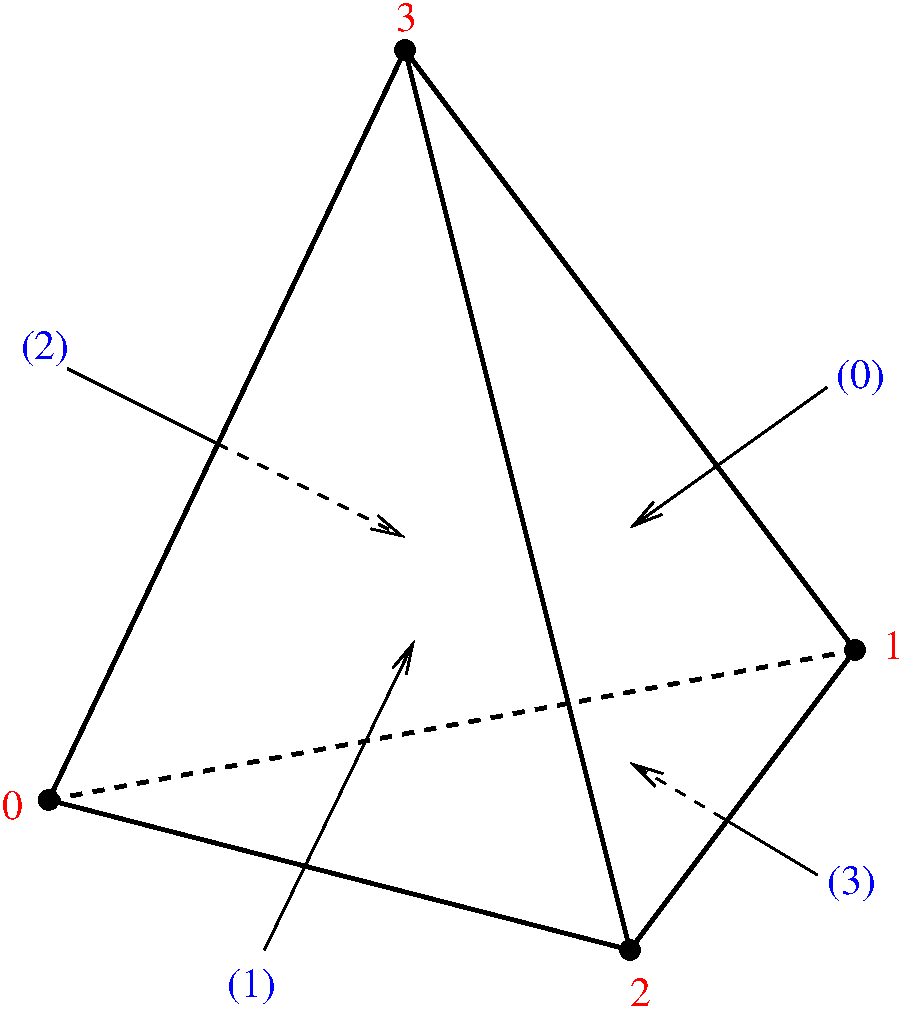
\includegraphics[scale=0.5]{tet-eps-converted-to.pdf}





\subsection{Source iteration}
The overall algorithm is to lag the data from the integral on the RHS of equation~\eqref{eq:main1}.
This is called source iteration
\begin{equation}
\Omega \cdot \nabla_x \Psi^{k+1} + \sigma_t \Psi^{k+1} = \frac{\sigma_s}{4\pi} \Phi^k + Q.
\end{equation}
Tycho 2 iterates this process until $||\Phi^{k+1} - \Phi^k||_\infty / ||\Phi^{k+1}||_\infty < \textrm{tolerance}$.



\subsection{Sweeps}
The most common method of solving the discretized form of equation~\eqref{eq:sweep} for $\Psi$ is called a sweep.
Consider the following 2D example shown below.

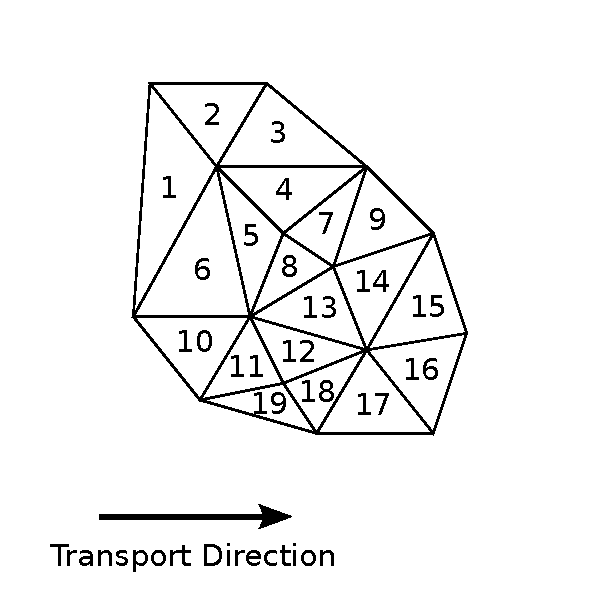
\includegraphics[scale=0.75]{grid2d.pdf}
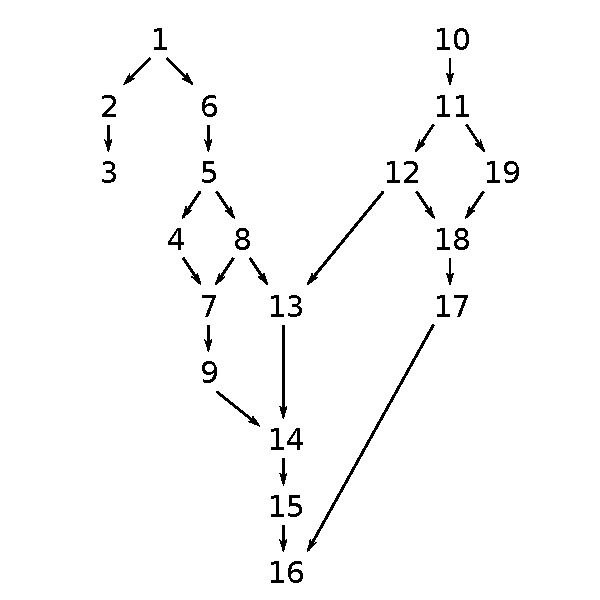
\includegraphics[scale=0.75]{dag.pdf}

The sweep algorithm for the transport direction (angle) shown, shows that cells 1 and 10 have no dependencies except for the incoming boundary.
Once $\Psi$ is computed in these cells, the upwind flux is calculated for the boundaries between (1,2), (1,6), and (10,11).
With this boundary data between cells known, $\Psi$ in cells 2, 6, and 11 can be computed.
This continues until $\Psi$ is computed in all cells.

A sweep is needed for each angle and energy group.
Fortunately, all these sweeps are completely independent and therefore trivially parallelizable.

\subsubsection{Sweeps Algorithms}
Several sweep algorithms have been employed.
The input deck currently allows 4 types of sweeps: {\tt OriginalTycho1}, {\tt OriginalTycho2}, {\tt GraphTraversal}, and {\tt PBJ}.
All but the {\tt PBJ} algorithm rely on each cell-angle pair having a priority assigned.
To understand why, consider the same sweep problem as shown in the previous figure but now split via MPI into 2 partitions.

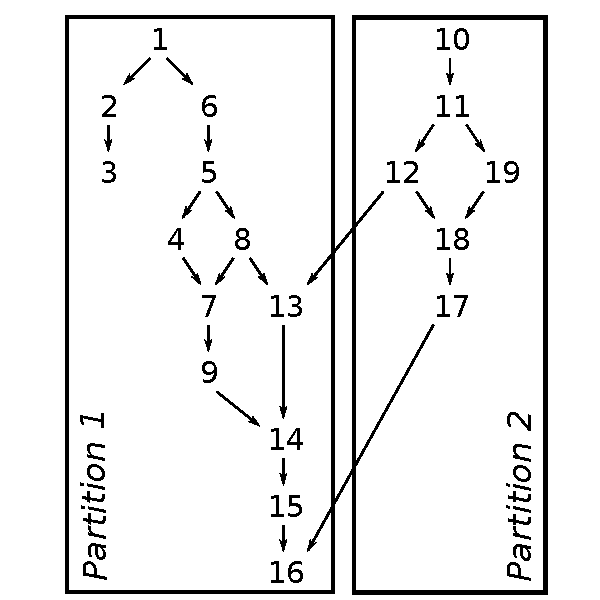
\includegraphics[scale=0.75]{dag_partitioned.pdf}

For partition 2, cell 10 must be computed first, then cell 11.
After this, there is a choice.
Either cell 12 or 19 can be computed, but cell 12 is probably best so that data can be communicated to compute cell 13 in partition 1.
Generally, the cell-angle priorities will attempt to get data to a partition boundary as quickly as possible.
The formulas for the priorities are detailed below but an explanation of the reasoning for each priority may be found in \cite{pautz-2002}.

\subsubsection{Intra-Angle Priorities}
Priorities are first created cells in each angle separately.
This is the definition of the intra-angle priorities.
Fundamental to all the priority calculations is the notion of B-Level of a cell.
This is defined to be the longest distance to leaf of the {\em entire} graph (not just for the partition).
For instance, node 17 has a B-Level of 1, node 16 has a B-Level of 0, and node 10 has a B-Level of 6 by traversing cells: 10, 11, 12, 13, 14, 15, 16.
Leaves of a graph have a B-Level of zero.

\paragraph{Random}
The random priority assigns a uniformly random priority to all cells.

\paragraph{B-Level}
The b-level priority assigns to each cell a priority equal to the cell's b-level.

\paragraph{BFDS}
This stands for Breadth First Descendant Seeking.
Each cell's priority is equal to the highest b-level of any descendant in another partition.
If there is no descendant in another partition, the priority is set to zero.

\paragraph{DFDS}
This stands for Depth First Descendant Seeking.
Each cell with a child in another partition has a priority equal to the maximum b-level of such children plus a constant equal or greater than the number of levels of the graph.
Parents are recursively assigned a priority of one less than the maximum of its children.
If a cell has no descendants in another partition, its priority is set to zero.

\paragraph{DFHDS}
This stands for Depth First Highest Descendant Seeking.
Each cell with a child in another partition has a priority equal to the maximum b-level of such children multiplied by (rather than addition as in DFDS) a constant equal or greater than the number of levels of the graph.
The rest of the algorithm is the same as for DFDS.

\subsubsection{Inter-Angle Priorities}
For a given cell, a priority is assigned for each angle independently via one of the intra-angle priorities above.
Now these priorities must be combined.

\paragraph{Interleaved}
For this priority type, the inter-angle priority is set to the intra-angle priority.
This can cause angles to be interleaved when cell-angle pairs are sorted by priority.

\paragraph{Globally Prioritized}
A sufficiently large constant is multiplied by the angle index to ensure a cell-angle pair with angle index less than another angle index has a lower priority.

\paragraph{Locally Prioritized}
First, for each angle, the maximum priority across cells is calculated to created an array of maximum priorities (with size of the number of angles).
The max priority array is sorted and angle indices are reordered with respect to the sorted max priority array.
Then the globally prioritized algorithm is used.


\subsubsection{The Sweep Algorithms}

The general sweep algorithm works as follows.
\begin{verbatim}
Assign priorities for each cell-angle pair
Calculate number of dependencies (parents) for each cell-angle pair
Place all cell-angle pairs with no dependencies in a priority queue
While (Still some cell-angle pair to compute)
  For i = 1 to maxCellsPerStep
    Pop cell-angle pair off priority queue
    Calculate Psi on cell-angle pair
    Update number of dependencies for children on MPI rank
    If (child has no dependencies)
      Put child in priority queue
    Send/Recv MPI rank's boundary data
    Update dependencies
    Place any cell-angle pairs with no dependencies in priority queue
\end{verbatim}


\paragraph{OriginalTycho 1 and 2}
Both of these sweep types use the same overall algorithm but differ on their OpenMP implementation.
In this section, the OpenMP implementation will not be discussed, and the text below equally describes both sweep types.

For this sweep type, the schedule of updates for $\Psi$ on each cell-angle pair is precomputed.
The for loop in the algorithm above is called a step and a queue of computational tasks is initially created for that loop.
Then, when it comes time to do the sweep, tasks are popped off the queue for each step.

\paragraph{GraphTraversal}
This sweep algorithm follows the above algorithm exactly.
In particular, the dependencies are updated calculated in real time for the sweep as opposed to precomputing them like the OriginalTycho algorithms.


\paragraph{PBJ}
PBJ stands for Parallel Block Jacobi.
In this algorithm, every MPI rank has an initial guess for the boundary data and a sweep is performed for each partition without regard for neighboring partitions.
Then boundary data is communicated between all MPI ranks and sweeps are performed on each individual partition again.
This is iterated until $\Psi$ does not change.



\begin{thebibliography}{1}

  \bibitem{pautz-2002} Shawn D. Pautz, ``An Algorithm for Parallel S$_n$ Sweeps on Unstructed Meshes,'' {\em Nuclear Science and Engineering}, 140, 111-136 (2002).

  

\end{thebibliography}













\end{document}